\documentclass{article}
\usepackage{fancyhdr}
\usepackage{titlesec}
\usepackage{graphicx}
\usepackage[dvipsnames]{xcolor}
\graphicspath{ {./img/} }

\pagestyle{fancy}
\fancyhf{}
\lhead{Modul 4 Praktikum Jaringan Komputer}
\rfoot{\footnotesize Page \thepage}
\lfoot{\footnotesize Mahyus Ihsan, S.Si, M.Si \newline Jurusan Informatika Universitas Syiah Kuala \newline Modul oleh : Diky Wahyudi, Furqan Al Ghifari, Rendika Rahmaturrizki}
\renewcommand{\headrulewidth}{1pt}
\renewcommand{\footrulewidth}{1pt}

\titleformat*{\section}{\small\bfseries}

\begin{document}
    \begin{center}
        \textbf{Modul 4 Praktikum Jaringan Komputer}

        \textbf{IPv4 dan Subnetting}
    \end{center}

    \section*{Deskripsi Singkat}
    IPv4 adalah singkatan dari \textbf{Internet Protocol Volume 4} yang memiliki fungsi sebagai pergantian berbagai jenis jaringan seperti Ethernet, atau yang lebih populer dengan sebutan Link layer Network.
    IPV4 terdiri dari berbagai jenis alamat yang tergolong menjadi tiga bagian, yakni unicast, multicast, dan broadcast. 
    Subnetting adalah teknik yang digunakan untuk memecahkan jaringan menjadi beberapa subjaringan yang lebih kecil.

    \section*{Tujuan}
    \begin{enumerate}
        \item Dapat memahami struktur dan jenis- jenis dari IPv4
        \item Dapat memahani tentang \textit{subnetting} dan implementasikan pengalamatan pada IPv4
        \item Dapat memahami dan melakukan \textit{Unicast dan Broadcast} pada IPv4 
    \end{enumerate}

    \begin{flushleft}
        \textbf{Materi 1 - Struktur dan Jenis - Jenis IPv4}
        \newline

        \textbf{IPv4} berukuran 32-bit yang dibagi menjadi 4 oktet dan setiap oktet terditi dari 8-bit. 
        1 bit sama dengan 1 digit angka biner 1/0. Jadi IPv4 dapat dituliskan dalam 2 cara :
        \begin{itemize}
            \item[] Dalam bentuk desimal \newline
            Contoh : 192.168.1.1
            \item[] Dalam bentuk biner \newline
            Contoh ; 11000000.10101000.00000001.00000001
        \end{itemize}

        \textbf{Subnetmask} merupakan sebuah teknik yang digunakan untuk membagi atau memecah jaringan komputer menjadi subnetwork dengan ukuran yang lebih kecil. Subnetmask juga berukuran 32-bit. \newline

        \textbf{Prefix} berfungsi sebagai penunjuk berapa banyak bit dari sebuah IP Address yang merupakan porsi Network Address. \newline
        Contoh : 192.168.1.0/24 , /24 adalah prefix. \newline

        \textbf{Porsi IP address} terbagi menjadi 3 bagian yaitu Network Address, Broadcast Address dan Host Address. \newline

        Contoh : 192.168.3.130/29 \newline
        Maka 29 angka pertama adalah Network-ID dan 3 angka sisanya adalah Host-ID, jadi banyaknya Host-ID yang tersedia adalah $2^3 = 8$ Host-ID dan host yang bisa digunakan adalah $8-2 = 6$, karena 2 buah host sudah digunakan oleh Network Address dan Broadcast Address.
        \begin{itemize}
            \item[] Network Address 11000000.10101000.00000011.10000\textcolor{red}{000} (Semua Nol) \newline 192.168.3.128
            \item[] Broadcast Address 11000000.10101000.00000011.10000\textcolor{red}{111} (Semua Satu) \newline 192.168.3.135
            \item[] Host Address adalah semua ip yang berada pada 192.168.3.128 sampai 192.168.3.135 dan host yang bisa digunakan adalah 192.168.3.129 sampai 192.168.3.134 yaitu 6.
        \end{itemize}
    \end{flushleft}

    \begin{flushleft}
        \textbf{Materi 2 - Melakukan Subnetting menggunakan Packet Tracer - Subnetting}
        \newline

        \begin{enumerate}
            \item Silahkan buka \textbf{Simulasi Modul 4.pkt} yang ada pada CiscoPacket.zip
            Dapat terlihat terdapat 4 buah PC, 2 buah Switch dan 1 buah Router.
            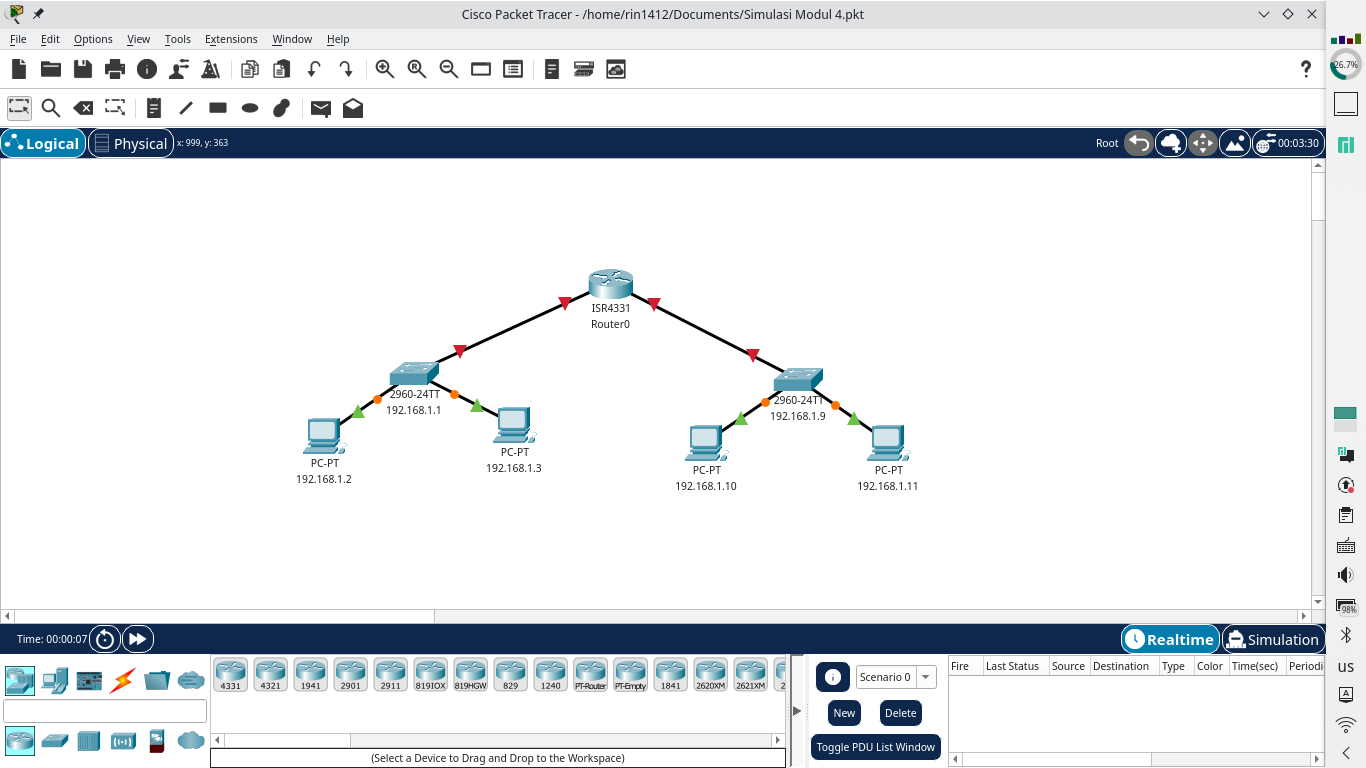
\includegraphics[scale=0.3]{2-1.png}

            \textbf{Berikut adalah IP dan Subnet yang akan digunakan dalam setiap device}

            \begin{tabular}{|c|c|c|c|}
                \hline
                Device & IP & Subnet & Network \\
                \hline
                Switch1 & 192.168.1.1 & 255.255.255.248 & 192.168.1.0 \\
                PC1 & 192.168.1.2 & 255.255.255.248 & 192.168.1.0 \\
                PC2 & 192.168.1.3 & 255.255.255.248 & 192.168.1.0 \\
                \hline
                Switch2 & 192.168.1.9 & 255.255.255.248 & 192.168.1.8 \\
                PC3 & 192.168.1.10 & 255.255.255.248 & 192.168.1.8 \\
                PC4 & 192.168.1.11 & 255.255.255.248  & 192.168.1.8 \\
                \hline
            \end{tabular}

            \item Selanjutnya lakukan pengaturan IP pada PC1 dan PC2, dengan cara klik pada PC1 \textbf{Desktop $>$ IP Configuration} kemudian masukkan IP dan Subnetmask nya.
            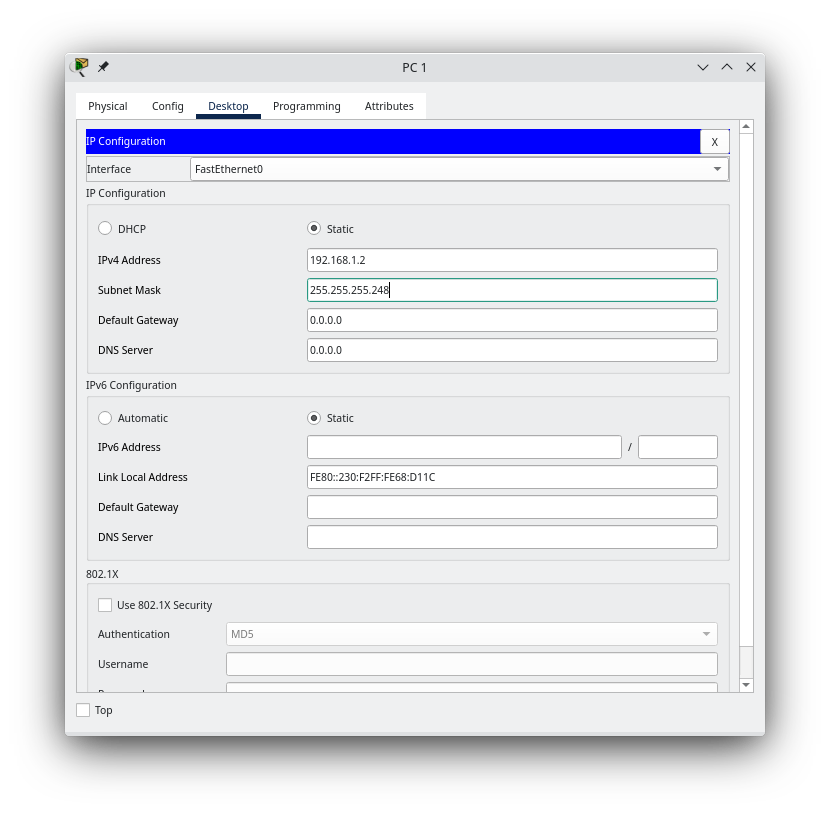
\includegraphics[scale=0.5]{2-pc1.png}
            Dan begitu juga dengan PC2 masukkan IP dan Subnetmasknya.

            \item Setelah itu uji konektivitas antara PC1 dan PC2, apakah sudah terhubung atau belum, yaitu dengan cara malakukan \textbf{ping} dari PC1 ataupun PC2.

            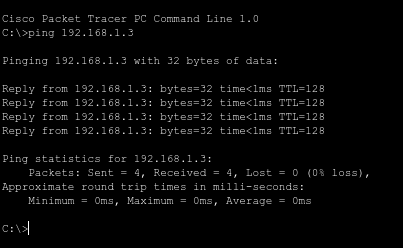
\includegraphics[scale=0.75]{2-ping-12.png}

            Terlihat bahwa \textbf{ping} telah berhasil dan mendapatkan \textbf{reply} dari alamat tujuan, maka PC1 dan PC2 sudah terhubung.

            \item Ulangi langkah 2 dan 3 pada PC3 dan PC4
            \item Maka kita telah berhasil menghubungkan PC yang berada di dalam network yang sama.
            \item Selanjutnya coba lakukan \textbf{ping} dari PC3 ke PC1, apakah PC3 mendapatkan \textbf{reply} dari PC1 ?
        \end{enumerate}
    \end{flushleft}

    \begin{flushleft}
        \textbf{Materi 3 - Melakukan Subnetting menggunakan Packet Tracer - Gateway}
        \newline

        \textbf{Gateway} adalah alat yang bertugas untuk menghubungkan berbagai perangkat komputer dengan protokol informasi yang berbeda.
        Selain itu, gateway juga bisa diartikan sebagai gerbang jaringan yang menghubungkan komputer dengan jaringan internet.

        \begin{enumerate}
            \item Setelah melakukan ping dari PC3 ke PC1, kita akan mendapatkan \textbf{Request time out} yang berarti ping kita tidak mendapatkan \textbf{reply} dari tujuan.
            
            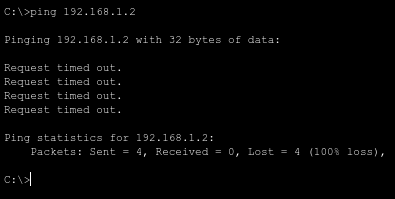
\includegraphics{3-ping-31.png}

            Hal ini dikarenakan karena kita belum menghubungkan Switch 1 dengan Switch 2 dan melakukan pengaturan \textbf{gateway}

            \item Untuk melakukan menghubungkan network 192.168.1.0 pada Switch 1 dengan network 192.168.1.8 pada Switch 2. Switch 1 dan 2 yang akan menjadi gateway nantinya.
            
            \item Pada router kita akan memberi IP pada \textbf{Switch 1 dan Switch 2} melalui router
            \item Pada Router0 silahkan buka menu CLI dan masuk kedalam \textbf{config terminal}
            
            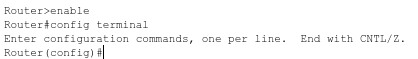
\includegraphics{3-gt-sw1-en.png}

            \item lalu kita akan melakukan pengaturan pada Switch 1 yang terhubung ke router melalui port \textbf{GigabitEthernet0/0/0} dan pada Swetch 2 yang terhubung ke router melalui port \textbf{GigabitEthernet0/0/1}
            
            Switch 1
            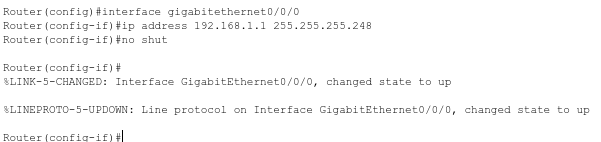
\includegraphics[scale=0.7]{3-setip-1.png} \newline

            Switch 2
            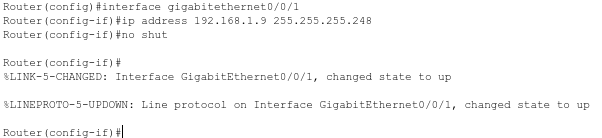
\includegraphics[scale=0.7]{3-setip-2.png} \newline

            note: perintah \textbf{no shut} (no shutdown) adalah perintah agar port tersebut menjadi hidup atau dalam status on.

            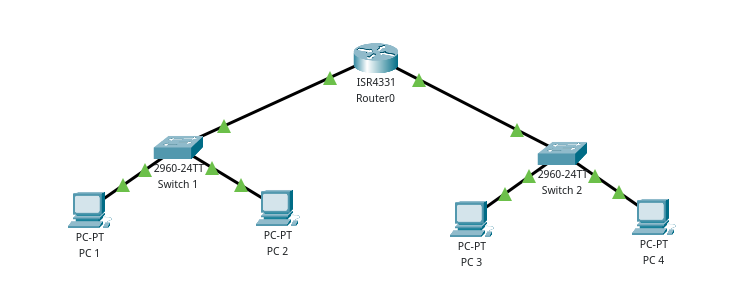
\includegraphics[scale=0.55]{3-connected.png}

            \item Sekarang kedua Network telah terhubung apakah kita sudah bisa berkomunikasi dengan device pada Network lain ? Tentu saja belum, karena kita belum memasukkan gateway pada PC 
            \item Untuk memasukkan gateway pada PC1 maka buka menu \textbf{Desktop $>$ IP Configuration} dan pada kolom bagian default gateway isikan IP dari Switch 1, Switch 1 berperan sebagai default gateway untuk Network 192.168.1.0 dan begtu juga pada PC2, dan pada PC3 dan PC4 masukkan IP Switch 2 sebagai default gateway dari Network 192.168.1.8
            \newpage

            Settingan pada PC1 
            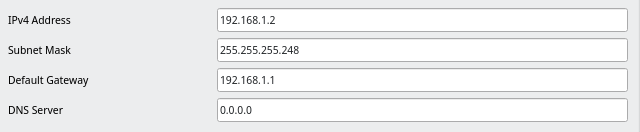
\includegraphics[scale=0.6]{3-pc1-ip.png} \newline

            Settingan pada PC2
            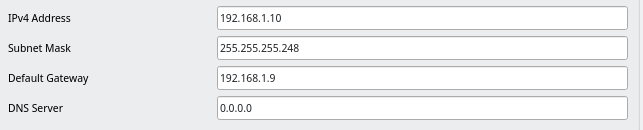
\includegraphics[scale=0.6]{3-pc3-ip.png}

            \item Sekarang lakukan kembali ping dari PC3 ke PC1 dan terlihat terdapat \textbf{reply} dari PC1. Berarti kedua network sudah terhubung dan semua komputer sudah bisa saling berkomunikasi.
            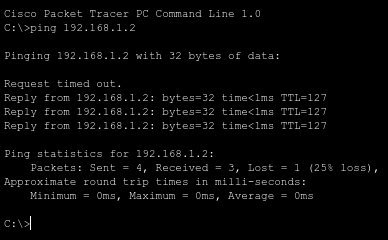
\includegraphics[]{3-ping-31-success.png}

            \item Sekarang coba tambahkan sebuah PC baru dengan nama PCNew pada Switch 2 dan lakukan konfigurasi IP agar PC tersebut agar bisa terkoneksi kepada semua PC.lainnya.
            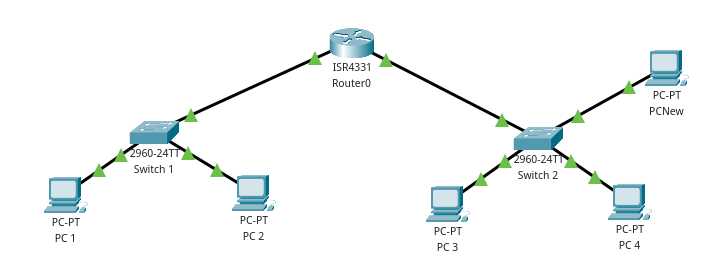
\includegraphics[scale=0.5]{3-newpc.png}
        \end{enumerate}
    \end{flushleft}

    \begin{flushleft}
        \textbf{Materi 4 - Melakukan \textit{unicast} dan \textit{broadcast}}
        \newline

        \textbf{Unicast} adalah transmisi satu-ke-satu dari satu titik di jaringan ke titik lain.
        \newline

        \textbf{Broadcast} adalah suatu metode pengiriman data, yang dimana data tersebut dikirim ke banyak titik sekaligus tanpa melakukan pemeriksaan atau pengecekan apakah titik tersebut siap atau tidak ataupun tanpa memperhatikan pakah data tersebut sampai atau tidak.
        \newline

        Untuk melakukan \textbf{\textit{Unicast}} dan \textbf{\textit{Broadcast}}
        \begin{enumerate}
            \item Masuk ke dalam mode Simulasi dan Klik Show All/None, kemudian masuk ke menu Edit Filter dan centang ICMP saja.
            \item Menggunakan jaringan yang telah kita buat sebelumnya pada Materi 2 dan 3, Untuk melakukan \textbf{\textit{Unicast}}, lakukan ping dari PCNew ke PC3, kemudian jalankan simulasi.

            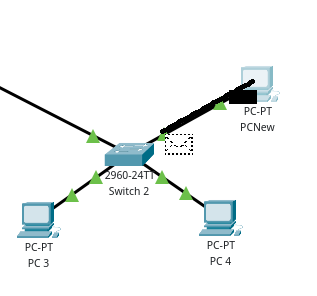
\includegraphics[scale=0.65]{4-sim1.png}
            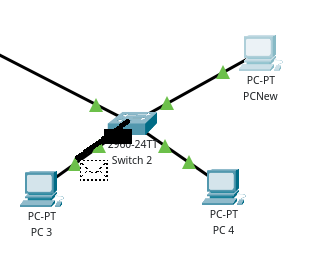
\includegraphics[scale=0.65]{4-sim2.png}

            Maka pesan dari PCNew hanya akan sampai kepada PC3 karena kita mengirimkan pesan ke IP PC3 yaitu 192.168.1.10

            \item Untuk melakukan \textbf{\textit{Broadcast}}, lakukan ping dari PCNew ke IP Broadcast pada Network tersebut yaitu 192.168.1.15, kemudian jalankan simulasi dan pesan akan dikirim kepada semua yang host yang berada di dalam Network tersebut.
            
            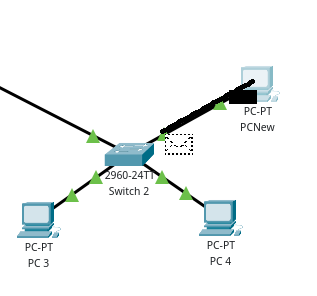
\includegraphics[scale=0.55]{4-sim1.png}
            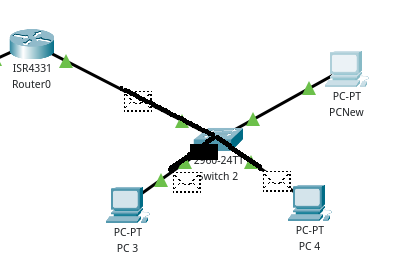
\includegraphics[scale=0.5]{4-sim3.png}
        \end{enumerate}
    \end{flushleft}

    \newpage
    \begin{flushleft}
        \textbf{Tugas}
        \newline

        \begin{enumerate}
            \item Silahkan tentukan Network Address, Broadcast Address, jumlah Host dan jumlah usable Host dari
            \begin{itemize}
                \item 192.168.1.130/29
                \item 198.168.1.64/25
            \end{itemize}
        \end{enumerate}
    \end{flushleft}
\end{document}
